%%----------------------------------------------------------------------------
%% Onderzoekstechnieken: Een bachelorproefvoorstel schrijven
%%----------------------------------------------------------------------------

\documentclass[aspectratio=169]{beamer}

%==============================================================================
% Aanloop
%==============================================================================

%---------- Vormgeving --------------------------------------------------------

\usetheme{hogent}

\usecolortheme{hgwhite} % witte achtergrond, zwarte tekst

\usepackage{graphicx,multicol}
\usepackage{comment,enumerate,hyperref}
\usepackage{amsmath,amsfonts,amssymb}
\usepackage[dutch]{babel}
\usepackage{multirow}
\usepackage{eurosym}
\usepackage{listings}
\usepackage{textcomp}
\usepackage{framed}
\usepackage{wrapfig}
\usepackage{tabu} %needed for \tabulinesep
\usepackage{wrapfig}
\usepackage{pgf-pie}
\usepackage{pgfplots}
\usepackage{booktabs}
\usepackage{pgfplotstable}
\usepackage{changepage}
\usepackage{ulem} % for \sout{text} (strikethrough)
\usepackage{fancyvrb} % for \begin{Verbatim} (LaTeX controls within verbatim)

%---------- Configuratie ------------------------------------------------------

\pgfplotsset{compat=1.16}
\usetikzlibrary{arrows,shapes,backgrounds,positioning,shadows,calc}
\usetikzlibrary{pgfplots.statistics}

%---------- Commando-definities -----------------------------------------------

\newcommand{\tabitem}{~~\llap{\textbullet}~~}
\newcommand{\alertbox}[2][hgblue]{%
  \setbeamercolor{alertbox}{bg=#1,fg=white}
  \begin{beamercolorbox}[sep=2pt,center]{alertbox}
    \textbf{#2}
  \end{beamercolorbox}
}
\pgfmathdeclarefunction{gauss}{2}{%
  \pgfmathparse{1/(#2*sqrt(2*pi))*exp(-((x-#1)^2)/(2*#2^2))}%
}

%---------- Bibliografie ------------------------------------------------------

\usepackage[backend=biber,style=apa]{biblatex}
\DeclareLanguageMapping{dutch}{dutch-apa}
\addbibresource{ozt-oef-1-latex.bib}

%---------- Info over de presentatie ------------------------------------------

\title{Rapporteren over onderzoek.}
\subtitle{Onderzoekstechnieken}
\author{Jens Buysse \and Wim {De Bruyn} \and Bert {Van Vreckem} \and Pieterjan Maenhaut}
\date{AJ 2020-2021}

%==============================================================================
% Inhoud presentatie
%==============================================================================

\begin{document}

\begin{frame}
  \maketitle
\end{frame}

\begin{frame}
  \frametitle{What's on the menu today?}
  
  \tableofcontents
\end{frame}


\section{Hoe rapporteren over onderzoek?}

\subsection{Fasen in het schrijven}

\begin{frame}
  \frametitle{Fasen in het schrijven}
  \centering
  \begin{tikzpicture}[
  auto,
  thick,
  ->,
  >=stealth',
  shorten >=1pt,
  node distance=1.2cm,
  fase/.style={ shape=rectangle, fill=hgblue!30, draw}]
  
  \node[fase] (1) {Planning};
  \node[fase] (2) [below of=1] {Organisatie};
  \node[fase] (3) [below of=2] {Kladversie};
  \node[fase] (4) [below of=3] {Ontwerp};
  \node[fase] (5) [below of=4] {Revisie};
  
  \draw (1) -- (2);
  \draw (2) -- (3);
  \draw (3) -- (4);
  \draw (4) -- (5);
  \end{tikzpicture}
\end{frame}

\begin{frame}
  \frametitle{Plannen van het document}
  
  \begin{description}
    \item[Waarom?] Doelstelling
    \item[Wie?] Wie is je publiek? Pas schrijfstijl en niveau aan!
    \item[Wat?] Inhoud: outline of mind map
    \item[Wanneer?] Hou rekening met tijdsbeperking, maak planning
    \item[Waar?] Omgeving
    \item[Hulpmiddelen?] Welke tools, software? Installeer deze!
  \end{description}
\end{frame}

\begin{frame}
  \frametitle{Het publiek}
  
  \begin{columns}[c]
    \column{.5\textwidth}
    
    \centering
    
    \textbf{De specialist}
    
    
\includegraphics[height=3cm]{oef2-04.png}
    
    \begin{itemize}
      \item Wil veel details zien
      \item Kent technische termen
    \end{itemize}
    
    \column{.5\textwidth}
    
    \centering
    
    \textbf{De niet-specialist}
    
    
\includegraphics[height=3cm]{oef2-05}
    
    \begin{itemize}
      \item Meer achtergrond, interpretatie nodig
      \item Non-technische termen nodig
      \item Wil technische termen uitgelegd zien
    \end{itemize}
  \end{columns}
\end{frame}

\begin{frame}
  \frametitle{Het publiek: enkele tips}
  
  Technische termen vs. jargon
  
  \begin{itemize}
    \item Technische termen: eigen aan vakgebied, kan je verduidelijken
    \item Jargon: luiheid, indruk willen maken
  \end{itemize}
  
  \vfill
  
  \centering
  
  \textcolor{hgorange}{$\times$ De PS3 heeft 6 $\times$ SPE @3.2GHz}
  
  vs.
  
  \textcolor{hgdarkgreen}{$\checkmark$ De Playstation 3 heeft 6 \textbf{Synergistic Processing Elements} met een snelheid van 3.2 GHz.}
\end{frame}

\begin{frame}
  \frametitle{Het publiek: enkele tips}
  
  \begin{itemize}
    \item Leg afkortingen uit
    \item Gebruik lijst van afkortingen indien nodig (en wees dan volledig!)
  \end{itemize}
  
  \vfill \centering
  
  \textbf{IP =}
  
  Internet Protocol?
  
  Intellectual Property?
  
  Interpersoonlijk?
  
  In Progress?
  
  enz.
  
  (\url{http://www.acronymfinder.com/IP.html})
  
\end{frame}

\begin{frame}
  \frametitle{Het publiek: enkele tips}
  
  Voeg conclusies expliciet toe (aparte sectie)
  
  \begin{itemize}
    \item Wordt vaak het eerst gelezen
    \begin{itemize}
      \item Uithangbord van je werk!
    \end{itemize}
    \item Ook al kan je publiek zelf conclusies maken
    \begin{itemize}
      \item Daarom gaan ze het nog niet doen
      \item Andere interpretaties mogelijk
      \item Jij bent de specialist, niet zij
    \end{itemize}
  \end{itemize}
\end{frame}

\subsection{Structuur van een document}

\begin{frame}[plain]
  \frametitle{Documentstructuur}
  
  \begin{columns}
    \column{.5\textwidth}
    \begin{center}
      Traditionele aanpak:
      
      \begin{tikzpicture}[auto,thick,->,>=stealth',
      shorten >=1pt, node distance=2.3cm,
      fase/.style={shape=rectangle,inner sep=8pt,fill=hgorange,draw}]
      
      \node[fase] (1) {Hoe aangepakt};
      \node[fase] (2) [below of=1] {Resultaten};
      \node[fase] (3) [below of=2] {Conclusies};
      
      \draw (1) -- (2);
      \draw (2) -- (3);
      
      \end{tikzpicture}
    \end{center}
    \column{.5\textwidth}
    \begin{center}
      Selectieve aanpak:
      
      \begin{tikzpicture}[auto,thick,->,>=stealth',
      shorten >=1pt, node distance=2.3cm,
      fase/.style={shape=rectangle,inner sep=8pt,fill=hgdarkgreen,draw}]
      
      \node[fase] (1) {Conclusies};
      \node[fase] (2) [below of=1] {Resultaten};
      \node[fase] (3) [below of=2] {Hoe aangepakt};
      
      \draw (1) -- (2);
      \draw (2) -- (3);
      
      \end{tikzpicture}
    \end{center}
  \end{columns}
\end{frame}

\begin{frame}
  \frametitle{Workflow $\ne$ volgorde tekst}
  
  Lezers zijn geïnteresseerd in motivatie en conclusies van je werk, meestal niet in details aanpak.
  
  \vfill
  
  \begin{columns}
    \column{.25\textwidth}
    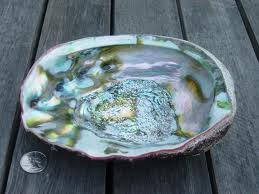
\includegraphics[width=\textwidth]{oef2-06}
    
    \column{.75\textwidth}
    \begin{quotation}
      Inspired by an abalone shell, Angela Belcher programs viruses to make elegant nanoscale structures that humans can use. Selecting for high-performing genes through directed evolution, she’s produced viruses that can construct powerful new batteries, clean hydrogen fuels and record-breaking solar cells.
    \end{quotation}
  \end{columns}
\end{frame}

\begin{frame}
  \frametitle{Documentstructuur}
  \framesubtitle{Kort document}
  
  \begin{columns}
    \column{.5\textwidth}
    \centering
    \begin{tikzpicture}[auto,thick,
    deel/.style={shape=rectangle,fill=hgdarkgreen,
      minimum width=4cm,draw}
    ]
    
    \node[deel] (1) [minimum height=24pt] {Introductie};
    \node[deel] (2) [below=6pt of 1,minimum height=56pt,fill=hgblue] {Corpus/body};
    \node[deel] (3) [below=6pt of 2,minimum height=24pt] {Conclusies};
    
    \end{tikzpicture}
    
    \column{.5\textwidth}
    \centering
    \begin{tikzpicture}[auto,thick,
    deel/.style={ shape=rectangle,fill=hgdarkgreen,
      minimum width=4cm,draw}]
    
    \node[deel] (1) [minimum height=24pt] {Voorwoord};
    \node[deel] (2) [below=6pt of 1,minimum height=24pt] {Samenvatting};
    \node[deel] (3) [below=6pt of 2,minimum height=56pt,fill=hgblue] {Corpus/body};
    \node[deel] (4) [below=6pt of 3,minimum height=24pt] {Conclusies};
    
    \end{tikzpicture}
    
  \end{columns}
\end{frame}

\begin{frame}[plain]
  \frametitle{Documentstructuur}
  \framesubtitle{Lang document}
  
  \begin{columns}
    \column{.5\textwidth}
    \centering
    \begin{tikzpicture}[auto,thick,
    deel/.style={ shape=rectangle,fill=hgdarkgreen,
      minimum width=4cm,draw}]
    
    \node[deel] (1) [minimum height=24pt] {Abstract};
    \node[deel] (2) [below=6pt of 1,minimum height=24pt] {Introductie};
    \node[deel] (3) [below=6pt of 2,minimum height=56pt,fill=hgblue] {Corpus/body};
    \node[deel] (4) [below=6pt of 3,minimum height=24pt] {Conclusies};
    \end{tikzpicture}
    
    \column{.5\textwidth}
    \centering
    \begin{tikzpicture}[auto,thick,
    deel/.style={ shape=rectangle,fill=hgdarkgreen,
      minimum width=4cm,draw}]
    
    \node[deel] (1) [minimum height=24pt] {Voorwoord};
    \node[deel] (2) [below=6pt of 1,minimum height=24pt] {Samenvatting};
    \node[deel] (3) [below=6pt of 2,minimum height=24pt] {Introductie};
    \node[deel] (4) [below=6pt of 3,minimum height=56pt,fill=hgblue] {Corpus/body};
    \node[deel] (5) [below=6pt of 4,minimum height=24pt] {Conclusies};
    \end{tikzpicture}
    
  \end{columns}
\end{frame}

\begin{frame}
  \frametitle{Documentstructuur}
  
  Voorwoord
  
  \begin{description}
    \item[Context] Waarom is dit werk belangrijk?
    \item[Nood] Waarom moest dit onderzocht worden?
    \item[Taak] Wat heb je uiteindelijk gedaan?
    \item[Object] Wat staat in dit document geschreven?
  \end{description}
  
  Samenvatting (abstract)
  
  \begin{description}
    \item[Resultaat] Wat staat in dit werk?
    \item[Conclusie] Relevantie voor publiek
    \item[Perspectief] Wat zegt de toekomst
  \end{description}
  
  (kort werk = 1 paragraaf, lang werk = max.~1 blz.)
\end{frame}

\begin{frame}[plain]
  %\frametitle{Voorbeeld voorwoord/samenvatting (abstract)}
  
  \begin{center}
    \only<1>{Context}
    \only<2>{Nood}
    \only<3>{Taak}
    \only<4>{Object}
    \only<5>{Resultaat+Conclusie}
  \end{center}
  
  \scriptsize
  \textbf{Energy-Efficient Resource Provisioning Algorithms for Optical Clouds}
  
  \alert<1>{Rising energy costs and climate change have led to an increased concern for energy-efficiency (EE).} \alert<2>{As Information and Communication Technology (ICT) is responsible for about 4\% of total energy consumption worldwide, it is essential to devise policies aimed at reducing it.} \alert<3>{In this paper, we propose a routing and scheduling algorithm for a cloud architecture, which targets minimal total energy consumption by enabling switching off unused network and/or Information Technology (IT) resources, exploiting the cloud-specific anycast principle.} \alert<4>{A detailed energy model for the entire cloud infrastructure comprising wide area optical network and IT resources is provided. This model is used to make a single-step decision on which IT end points to use for a given request, including the routing of the network connection towards these end points. Our simulations quantitatively assess the EE algorithm’s potential energy savings, but also assess the influence this may have on traditional Quality of Service parameters such as service blocking. Furthermore, we compare the one-step scheduling with traditional scheduling and routing schemes, which calculate the resource provisioning in a two-step approach (selecting first the destination IT end point, and subsequently using unicast routing towards it).} \alert<5>{We show that depending on the offered infrastructure load, our proposed one step calculation considerably lowers the total energy consumption (reduction up to 50\%) compared to the traditional iterative scheduling and routing, especially in low to medium load scenarios, without any significant increase in the service blocking.}
  
\end{frame}

\section{Hoe refereren naar vakliteratuur?}

\subsection{Waarom een literatuurstudie?}

\begin{frame}
  \frametitle{Vaak voorkomende fouten}
  
  \begin{itemize}
    \item Onvolledige/geen referentielijst
    \item Enkel URLs
    \item Te weinig informatie in referentielijst
    \begin{itemize}
      \item $\Rightarrow$ bronnen niet terug te vinden
    \end{itemize}
    \item Onaanvaardbare bronnen
    \item Verkeerde opmaak
    \item Geen verwijzingen naar bronnen vanuit de tekst
    \item Opgedeeld per type (boek, web, enz.)
  \end{itemize}
\end{frame}

\begin{frame}
  \frametitle{Doel van de literatuurstudie}
  
  \begin{itemize}
    \item Inleiding op onderwerp
    \item Wat is de huidige stand van zaken?
    \item Wat zeggen experts er over?
    \item Onderzoeksvragen verduidelijken, in context plaatsen
    \item Er is een probleem dat een oplossing vraagt
  \end{itemize}
  
  \bigskip
  
  \alertbox{\textcolor{hgyellow}{Elke bewering} in een literatuurstudie moet je bewijzen a.h.v.~referenties}
\end{frame}

\begin{frame}
  \frametitle{Doel van de referentielijst}
  
  Lezers toelaten:
  
  \begin{itemize}
    \item De gerefereerde bronnen op te zoeken
    \item Waarde bronnen zelf te beoordelen
  \end{itemize}
  
  \pause
  
  Strikte, vastgelegde vorm:
  
  \begin{itemize}
    \item Vastgelegde regels, afh.~publicatie (bv. IEEE, APA, Chicago Manual of Style, \ldots)
    \item Vaste volgorde (volgorde in de tekst of alfabetisch)
    \item Lijst URLs is onvoldoende!
  \end{itemize}
  
  \pause
  
  \alertbox{Gebruik \textcolor{hgyellow}{referentie-software} om je referentielijst op te maken!}
\end{frame}

\begin{frame}
  \frametitle{Wanneer refereren naar de literatuur?}
  
  \begin{itemize}
    \item Definities, eerste vermelding vakterm
    \item Overnemen uit bron van letterlijk citaat, vertaling/parafrase, of afbeelding
    \begin{itemize}
      \item Geen referentie = \alert{plagiaat!}
    \end{itemize}
    \item Aanhalen resultaten vorig onderzoek
    \item Vrijwel elke bewering die je doet over het vakgebied
  \end{itemize}
  
  \bigskip
  
  \alertbox{Referenties geven \textcolor{hgyellow}{geloofwaardigheid} aan je literatuurstudie}
\end{frame}

\subsection{Informatie opzoeken en bijhouden}

\begin{frame}
  \frametitle{Soorten bronnen}
  
  \begin{description}
    \item[Primaire] Kennis die je \textbf{zelf vergaart} tijdens onderzoek
      
      Experimenten, enquêtes, interviews, \ldots

    \item[Secundaire] \textbf{Publicatie} van kennis, onderzoek, \ldots door anderen
    
      Artikel in wetenschappelijke journal of vaktijdschrift, presentatie op conferentie, boek, \ldots

    \item[Tertiaire] \textbf{Indexen}

      Zoekmachine, encyclopedie, databank bibliotheek, \ldots

  \end{description}
  
  \alertbox{Enkel \textcolor{hgyellow}{secundaire bronnen} zijn bruikbaar als referenties.}
\end{frame}

\begin{frame}
  \frametitle{Informatie opzoeken}
  
  Start bij \alert{tertiare} bronnen:
  
  \begin{itemize}
    \item Google Scholar: \url{https://scholar.google.com/}
    \item ScienceDirect: \url{https://www.sciencedirect.com/}
    \item Springer Online Journals: \url{https://link.springer.com/}
    \item Catalogus Bib: \url{https://www.hogent.be/student/bibliotheken/}
    \item Wikipedia (uiteraard\dots)
  \end{itemize}
  
  \alertbox{Let op: tertiare bronnen, ihb.~Wikipedia, zijn zelf \textcolor{hgyellow}{niet} aanvaardbaar als referentie}
  
  \pause
  
  \begin{itemize}
    \item Geen garantie op juistheid
    \item Beweringen niet altijd aangetoond: [citation needed]
    \item \alert{Wél} een goed startpunt (bv. referenties onderaan artikel)
  \end{itemize}
\end{frame}

\begin{frame}
  \frametitle{Tips}
  
  \begin{itemize}
    \item<+-> Bezoek website HOGENT \textbf{bib}: \url{https://www.hogent.be/student/bibliotheken/}
    \begin{itemize}
      \item Zoeken, Scripties/Taken, Databanken
      \item Cursus Informatievaardigheden (\url{https://chamilo.hogent.be/index.php?go=CourseViewer\&application=Chamilo\%5CApplication\%5CWeblcms\&course=22068\&tool=LearningPath\&browser=Table\&tool_action=ComplexDisplay\&publication=980981})
    \end{itemize}
    \item<+-> \textbf{Apollox} (\url{https://apollox.hogent.be/})
    \begin{itemize}
      \item start applicaties/zoekmachines vanop HoGent
      \item vb.~SPSS, Endnote, Visio, Office
      \item Online journals en ebooks waar HoGent een abonnement voor heeft (bv.~ScienceDirect, SpringerLink)
    \end{itemize}
  \end{itemize}
\end{frame}

\begin{frame}
  \frametitle{Tips (vervolg)}
  
  \begin{itemize}
    \item<+-> \textbf{Google Scholar}
      \begin{itemize}
        \item Gebruik vanop de campus of via Apollo
        \item Kijk uit naar download-links aan de rechterkant: [PDF] of [fulltext@Hogent]
        \item Referentie in Bib{\TeX}-formaat verkrijgen (via instellingen)
        \item Gebruik zoekopties (bv.~beperken in tijd)
      \end{itemize}
    \item Presentaties \textbf{vakconferenties} (via Youtube, Vimeo, Slideshare, \dots)
    \begin{itemize}
      \item vb. Google IO, WWDC, FOSDEM, Velocity, \dots
      \item Zoeken via Lanyrd (\url{http://lanyrd.com/topics/})
    \end{itemize}
    \item<+-> Technische \textbf{portaalsites} voor ict-gerelateerde onderwerpen
    \begin{itemize}
      \item vb.~dzone.com, infoq.com, TechNet, enz.
    \end{itemize}
  \end{itemize}
\end{frame}

\begin{frame}
\frametitle{Tips (vervolg)}

\begin{itemize}
    \item<+-> Wie zijn de belangrijkste namen in de \textbf{community}?
    \begin{itemize}
      \item Keynotes op conferenties, auteurs van standaardwerken, enz.
      \item Volg ze op Twitter
      \item Zoek hun blog
    \end{itemize}
    \item<+-> \textbf{Technische blogs} van bedrijven
    \begin{itemize}
      \item Google Developers Blog, Twitter Engineering/Developer Blog, Netflix Tech Blog, \dots
    \end{itemize}
  \end{itemize}
\end{frame}


\begin{frame}
  \frametitle{Bruikbare bronnen}
  
  (Voor een bachelorproef Informatica)
  
  \begin{description}
    \item[Journal article]<+-> in wetenschappelijk, peer reviewed tijdschrift
    \item[Conference proceedings]<+-> artikel gepresenteerd op wetenschappelijk, peer reviewed congres
    \item[Thesis]<+-> doctoraat (PhD), Master, evt.~Bachelor
    \item[Handleiding]<+-> bv.~van gebruikte of besproken software
    \item[Boek]<+-> let op: iedereen kan een boek uitgeven. Controleer auteur, uitgeverij, doelpubliek (Springer vs. ``for dummies'')
    \item[Presentatie]<+-> door erkend vakexpert, bv.~op vakconferentie (via Youtube, Vimeo, enz.)
    \item[Blogartikel]<+-> indien geschreven door erkend vakexpert
    \item[Vaktijdschrift]<+-> let op: geschreven door journalist (is geen vakexpert)
  \end{description}
\end{frame}

\begin{frame}
  \frametitle{Onbruikbare bronnen}
  
  \begin{itemize}
    \item Eender welk werk zonder auteur of publicatiejaar
    \item Wikipedia-artikel
    \item Blogartikel van iemand buiten het vakgebied
    \item ``White papers'' (meestal niet objectief)
    \item Homepage van een besproken product of bedrijf
    \begin{itemize}
      \item Evt.~in de tekst zelf of als voetnoot
    \end{itemize}
    \item \dots
  \end{itemize}
\end{frame}

\begin{frame}
  \frametitle{Checklist kwaliteit bronnen}
  \framesubtitle{Doe de CRAP test}
  
  \begin{description}
    \item[Current] Publicatiejaar? Is het voldoende recent? Is dit nog conform de \textbf{state-of-the-art}?
    \item[Reliable] Is het objectief? Gebalanceerd of eenzijdig? 
    Bronvermeldingen?
    \item[Authoritative] Auteur? Is dit een erkend expert? Wordt er elders naar verwezen?
    \item[Purpose/Point of View] Opinie of feiten? Wil de auteur iets verkopen? Is het relevant voor je onderzoeksvraag?
  \end{description}
  
\end{frame}

\begin{frame}[fragile]
  \frametitle{Bronvermelding en referentielijst in {\LaTeX}}
  
  Bib{\LaTeX} en Biber
  
  \vspace{18pt}
  
  \verb|artikel.tex|: Hoofdtekst\\
  \verb|artikel.bib|: Bibliografische databank (bewerk met bv.~JabRef)
  
  \vspace{18pt}
  
  Preamble:
  
  \begin{verbatim}
  \usepackage[backend=biber,style=apa]{biblatex}
  \DeclareLanguageMapping{dutch}{dutch-apa}
  \addbibresource{artikel.bib}
  \end{verbatim}
  
\end{frame}

\begin{frame}
  \frametitle{Bibliografische gegevens in Jabref}
  
  Info die \textbf{altijd} ingevuld moet worden:
  
  \begin{description}
    \item[Author] Familienaam, Voornaam and Familienaam, Voornaam and Familienaam, Voornaam\ldots
    \item[Title] v/h artikel, boek, \ldots
    \item[Year] of datum van publicatie
    \item[Bibtexkey] id van deze bron, gebruikt bij refereren (tip: klik op sleutel-icoon)
  \end{description}
\end{frame}

\begin{frame}[fragile]
  \frametitle{Bibliografische gegevens in Jabref}
  \framesubtitle{Extra info voor Article}
  
  \begin{description}
    \item[Journal] Naam van het tijdschrift
    \item[Volume] Jaargang
    \item[Number] Nummer binnen de jaargang (optioneel)
    \item[Pages] \verb|mmm--nnn|
  \end{description}

  \bigskip
  
  \textbf{Voorbeeld:}
  
  \bigskip
  
  \fullcitebib{Anscombe1973}
\end{frame}

\begin{frame}
  \frametitle{Bibliografische gegevens in Jabref}
  \framesubtitle{Extra info voor Electronic}
  
  \begin{description}
    \item[Url] Hyperlink naar de bron
    \item[Urldate] Datum van raadplegen
  \end{description}

  \bigskip

  \textbf{Voorbeeld:}

  \bigskip

  \fullcitebib{Lundin2020}

\end{frame}

\begin{frame}
  \frametitle{Bibliografische gegevens in Jabref}
  \framesubtitle{Extra info voor InProceedings}
  
  \begin{description}
    \item[Booktitle] ``Proceedings of the [naam conferentie]''
    \item[Editor] Redacteur(s) (optioneel)
    \item[Pages] paginanummers (optioneel)
  \end{description}
  
  \medskip
  
  \textbf{Voorbeeld:}
  
  \fullcitebib{vanderLaanEtAl2015}
\end{frame}

\begin{frame}
  \frametitle{Bibliografische gegevens in Jabref}
  
  Vul zoveel mogelijk info in (maakt zoeken gemakkelijker):
  
  \begin{description}
    \item[DOI] Digital Object Identifier: uniek ID voor artikel, hiermee kan je automatisch alle velden invullen
    \item[URL] ook al is het niet echt een Electronic bron
    \item[Keywords] Sleutelwoorden
    \item[File] PDF van de publicatie
    \item[Abstract] Samenvatting
    \item[Comments] Je eigen samenvatting/opmerkingen
  \end{description}
  
\end{frame}

\begin{frame}[fragile]
  \frametitle{Bronvermelding en referentielijst in {\LaTeX}}
  
  \begin{itemize}
    \item Verwijzingen in de tekst:
    
    \begin{itemize}
      \item \verb|\textcite{Knuth1998}| $\Rightarrow$ Knuth (1998)
      \item \verb|\autocite{Knuth1998}| $\Rightarrow$ (Knuth, 1998)
    \end{itemize}
    
    \item Literatuurlijst invoegen: \verb|\printbibliography|
    
    \item Compileren (in TexStudio):
    
    \begin{enumerate}
      \item Build/Compile (F5 of F6): bronnen worden nog niet toegevoegd, ``keys'' van bronnen in het vet aangeduid
      \item Bibliography (F8): selecteert de gerefereerde bronnen en maakt ze klaar
      \item Build/Compile (F5 of F6): effectief invoegen verwijzingen en literatuurlijst
    \end{enumerate}
  \end{itemize}
  
  Zie de voorziene sjablonen of de cursus voor voorbeelden!
\end{frame}

\begin{frame}
  \frametitle{Oefening}
  
  \begin{itemize}
    \item Compileer de cursus Onderzoekstechnieken in TexStudio en controleer of het lukt de bibliografie en bronverwijzingen in te voegen (F5 - F8 - F5)
    \item Zoek een aantal artikels i.v.m.~onderwerp van de groepstaak
    \item Voer ze in in JabRef
    \begin{itemize}
      \item Hou zo veel mogelijk informatie bij (ook bv. abstract, keywords, PDF, URL)
    \end{itemize}
    \item Voeg vultekst met referenties en literatuurlijst toe aan het sjabloon voor het artikel
  \end{itemize}
\end{frame}

\begin{frame}
  \frametitle{Meer info}
  
  De inhoud van deze les is verwerkt in een ``Praktische gids voor de bachelorproef''
  
  \vspace{12pt}
  
  \url{https://github.com/HoGentTIN/bachproef-gids/releases}
  
\end{frame}

\end{document}